% !TeX program = pdflatex
% Complete manuscript. The figures are drawn in TikZ.
% Compile with latexmk -pdf book-en.tex.
\documentclass[12pt,oneside]{article}
\usepackage[T1]{fontenc}
\usepackage[utf8]{inputenc}
\usepackage[sc]{mathpazo}
\usepackage{amsmath,amssymb,booktabs,microtype}
\usepackage[paperwidth=165mm,paperheight=235mm,left=22mm,right=21mm,top=22mm,bottom=24mm,headheight=14pt,headsep=7mm,footskip=12mm]{geometry}
\usepackage{xcolor,tikz,fancyhdr,titlesec,needspace,environ}
\usepackage[unicode,hidelinks]{hyperref}
\hypersetup{pdfauthor={Caio Gomes},pdftitle={The CAIO Lectures on Machine Learning},pdfsubject={How to Think About Machine Learning. Probability updates and classification.},pdflang={en},bookmarksopen=true,bookmarksnumbered=false,pdfdisplaydoctitle=true}
\definecolor{tinta}{HTML}{224D50}
\definecolor{leve}{HTML}{B9CFCC}
\definecolor{papel}{HTML}{F4F7F6}
\urlstyle{same}
\pagestyle{fancy}\fancyhf{}
\fancyhead[R]{\footnotesize\itshape\nouppercase{\rightmark}}\fancyfoot[C]{\small\thepage}
\renewcommand{\headrulewidth}{0pt}
\fancypagestyle{opening}{\fancyhf{}\fancyfoot[C]{\small\thepage}\renewcommand{\headrulewidth}{0pt}}
\setlength{\parindent}{1em}\setlength{\parskip}{4pt plus 1pt minus 1pt}\linespread{1.16}
\renewcommand{\arraystretch}{1.12}
\setlength{\emergencystretch}{1.7em}
\interfootnotelinepenalty=10000\clubpenalty=10000\widowpenalty=10000\displaywidowpenalty=10000
\titleformat{\subsection}{\large\bfseries}{}{0pt}{}
\titlespacing*{\subsection}{0pt}{18pt plus 4pt minus 3pt}{8pt}
\setcounter{secnumdepth}{0}\raggedbottom
\newcommand{\F}{\mathcal F}
\newcommand{\alinhamentodotitulo}{\raggedright}
\newcommand{\capitulo}[2]{\clearpage\thispagestyle{opening}\markright{#2}\phantomsection\label{chapter:#1}\pdfbookmark[0]{Chapter #1 · #2}{ch#1}\noindent{\small\color{tinta}\textsc{Chapter #1}\par}\vspace{8pt}{\alinhamentodotitulo\noindent\fontsize{24}{27}\selectfont\bfseries #2\par}\vspace{18pt}\noindent\ignorespaces}
\newcommand{\secao}[1]{\Needspace{5.2\baselineskip}\subsection*{#1}}
\newcommand{\itemq}[1]{\par\textbf{#1.}\enspace}
\NewEnviron{quadro}[1]{\par\addvspace{12pt}\begingroup\setlength{\fboxsep}{10pt}\setlength{\fboxrule}{.55pt}\noindent\fcolorbox{tinta}{papel}{\begin{minipage}{\dimexpr\linewidth-2\fboxsep-2\fboxrule\relax}\small\setlength{\parindent}{0pt}\setlength{\parskip}{4pt}{\large\bfseries\color{tinta}#1\par}\vspace{3pt}\BODY\end{minipage}}\par\endgroup\addvspace{12pt}}
\newcommand{\mesas}{%
\par\addvspace{7pt}\noindent\begin{minipage}{\linewidth}\centering

\begin{tikzpicture}[x=.42cm,y=.44cm,font=\small]
\node[anchor=east] at (-.32,1.49) {Coin A};
\node[anchor=east] at (-.32,.29) {Coin B};
\foreach \j in {0,...,15}{
 \ifnum\j<9 \def\filla{tinta}\else\ifnum\j<12 \def\filla{leve}\else\def\filla{white}\fi\fi
 \ifnum\j<1 \def\fillb{tinta}\else\ifnum\j<4 \def\fillb{leve}\else\def\fillb{white}\fi\fi
 \filldraw[fill=\filla,draw=tinta, line width=.35pt] (\j,1.04) rectangle +(0.87,.87);
 \filldraw[fill=\fillb,draw=tinta, line width=.35pt] (\j,-.16) rectangle +(0.87,.87);
}
\end{tikzpicture}\par\vspace{2pt}
{\footnotesize\raggedright Each square stands for one table in the expected counts. The shaded tables got heads on the first toss. The dark ones also got heads on the second.\par}
\end{minipage}\par\addvspace{5pt}}
\newcommand{\perdasmargem}{%
\par\addvspace{7pt}\noindent\begin{minipage}{\linewidth}\centering
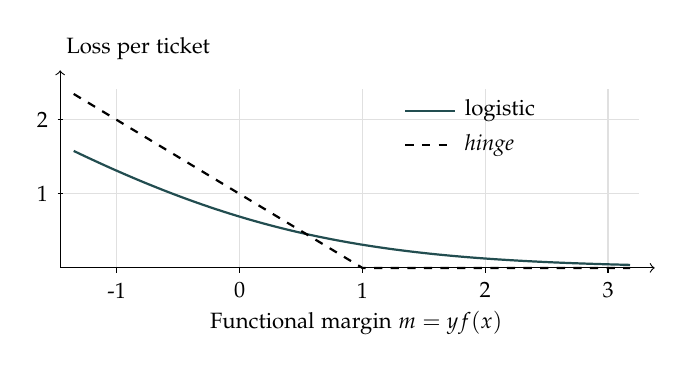
\begin{tikzpicture}[x=1.56cm,y=0.94cm,font=\footnotesize]
\foreach \x in {-1,0,1,2,3} {\draw[black!12] (\x,0)--(\x,2.42);\draw (\x,0)--(\x,-.07) node[below]{\x};}
\foreach \y in {1,2} {\draw[black!12] (-1.45,\y)--(3.25,\y);\draw (-1.48,\y)--(-1.44,\y) node[pos=0,left]{\y};}
\draw[->](-1.46,0)--(3.38,0);\draw[->](-1.46,0)--(-1.46,2.67);
\node[anchor=west] at (-1.49,2.97) {Loss per ticket};
\node at (.95,-.74) {Functional margin \(m=yf(x)\)};
\draw[tinta,thick,domain=-1.35:3.18,samples=100] plot (\x,{ln(1+exp(-\x))});
\draw[black,thick,dashed] (-1.35,2.35)--(1,0)--(3.18,0);
\draw[tinta,thick] (1.35,2.12)--(1.75,2.12) node[right,black]{logistic};
\draw[black,thick,dashed] (1.35,1.66)--(1.75,1.66) node[right,black]{\emph{hinge}};
\end{tikzpicture}\par
{\footnotesize\raggedright On both curves, a positive margin means the letter was identified correctly. With the \emph{hinge} loss, once \(m\) reaches 1, that example owes nothing.\par}
\end{minipage}\par\addvspace{7pt}}
